Problemy z którymi spotykamy się w praktyce są nierzadko z natury wielowymiarowe. W rozdziale \ref{sec:popularne_spready} opowiemy o clean dark spreadach, czyli mierze rentowności elektrowni węglowej który wymaga modelowania zależności trzech komponentów (ceny węgla, ceny certyfikatów emisyjnych i ceny energii). Model LDA dla ryzyka operacyjnego nadmieniony w rozdziale \ref{subsec:dwuwymiarowe_kopuly_przyklady} wymaga segmentacji strat względem przynależności do jednej z kilkunastu/kilkudziesięciu homogenicznych kategorii (ORC) i modelowania zależności między nimi. Natomiast modelowanie zależności komponentów portfela inwestycyjnego może okazać się nawet kilkusetwymiarowym problemem.\\
Widzimy więc, że przekrój zastosowań praktycznych jest bardzo duży i istnieje zapotrzebowanie na wielowymiarowe modele zależności. Dwuwymiarowe kopuły przedstawione w \ref{subsec:dwuwymiarowe_kopuly_przyklady} mają często swoje wielowymiarowe odpowiedniki (\cite{Cherubini_Copula_Methods_in_Finance}, \cite{Kurowicka_Dependence_Modeling}). Są one jednak stosunkowo mało elastyczne, ponieważ nie pozwalają ,,dostroić" modelu na poziomie interakcji każdej pary wymiarów zmiennej losowej. W tym rozdziale sięgniemy po modele Vine Copula, które pozwolą modelować wielowymiarowe zależności w dużych detalach, do stopnia gdzie będziemy w stanie określić zależność między dowolnymi dwoma rozkładami brzegowymi.\\

\subsection{Pair Copula Constructions}
\label{subsec:pair_copula_constructions}
Zaczniemy od przykładu w trzech wymiarach, aby zilustrować czym jest \emph{Pair copula construction} (PCC). Ogólną ideą jest aby wielowymiarowy rozkład zmiennej losowej rozbić na dwuwymiarowe komponenty modelowane za pomocą dwuwymiarowych kopuł.\\

W poniższych rozważaniach przydadzą nam się następujący lemat dotyczący relacji między gęstością kopuły a rozkładami warunkowymi:

\begin{lemma}
	Rozkład warunkowy dwuwymiarowej zmiennej losowej można przedstawić w języku kopuły:	
	$$ f_{1|2}(x_1|x_2) =c_{12}(F_1(x_1), F_2(x_2))f_2(x_2).$$
	\label{lem:copula_representation_of_conditional_density}
\end{lemma}
\begin{proof}
	Posługując się twierdzeniem Sklara \ref{thm:sklar_theorem_density} mamy:
	\begin{equation*}
		\begin{split}
			f_{1|2}(x_1, x_2) & = \frac{f_{12}(x_1, x_2)}{f_2(x_2)} \\
			& = \frac{c_{12}(F_1(x_1), F_2(x_2))f_1(x_1)f_2(x_2)}{f_2(x_2)}\\
			& = c_{12}(F_1(x_1), F_2(x_2))f_1(x_1)
		\end{split}
	\end{equation*}
\end{proof}

\subsubsection{Przykład ilustrujący}
\label{subsub:przyklad_3_wymiary}
Aby zilustrować PCC, rozpatrzmy rozkład $3$-wymiarowy o gęstości $f(x_1, x_2, x_3)$. Tę gęstość można przedstawić w postaci:

$$ f(x_1, x_2, x_3) = f_{3|12}(x_3|x_1, x_2)f_{2|1}(x_2|x_1)f_1(x_1).$$

Celem jest sfaktoryzowanie tego wyrażenia do postaci wykorzystującej co najwyżej dwuwymiarowe kopuły lub jednowymiarowe rozkłady brzegowe. Widzimy, że w tym celu należy rozwinąć $f_{3|12}$ oraz $f_{2|1}$. \\
Korzystając z lematu \ref{lem:copula_representation_of_conditional_density} otrzymujemy bezpośrednio $f_{2|1}$ oraz $f_{3|1}$ (które przyda się za chwilę) jako:
\begin{equation*}
	\begin{split}
		f_{1|2}(x_1|x_2) &= c_{12}(F_1(x_1), F_2(x_2))f_2(x_2),\\
		f_{3|2}(x_3|x_2) &= c_{32}(F_3(x_3), F_2(x_2))f_2(x_2)
	\end{split}
\end{equation*}

Natomiast w celu otrzymania $f_{3|12}$ będziemy musieli przejść przez dwuwymiarowy rozkład $f_{13|2}(x_1, x_3|x_2)$. Ma on rozkłady brzegowe $F_{1|2}(x_1|x_2)$ oraz $F_{3|2}(x_3|x_2)$ i kopułę warunkową $c_{13;2}$~-~czyli kopułę rozkładu $(X_1, X_3) | X_2=x_2$. Zaaplikujemy do niego twierdzenie Sklara \ref{thm:sklar_theorem_density}:

\begin{equation*}
	\begin{split}
		f_{3|12}(x_3|x_1,x_2)  & = \frac{f_{13|2}(x_1, x_3|x_2)}{f_{1|2}(x_1|x_2)} \\
		& = \frac{c_{13;2}(F_{1|2}(x_1|x_2), F_{3|2}(x_3|x_2); x_2)f_{1|2}(x_1|x_2)f_{3|2}(x_3|x_2)}{f_{1|2}(x_1|x_2)}\\
		& = c_{13;2}(F_{1|2}(x_1|x_2), F_{3|2}(x_3|x_2); x_2)f_{3|2}(x_3|x_2) \\
		& = c_{13;2}(F_{1|2}(x_1|x_2), F_{3|2}(x_3|x_2); x_2)c_{32}(F_3(x_3), F_2(x_2))f_2(x_2)
	\end{split}
\end{equation*}

Finalnie otrzymujemy dekompozycję $f(x_1, x_2, x_3)$ do postaci:

\begin{equation}
	\begin{split}
	f(x_1, x_2, x_3) = &c_{13;2}(F_{1|2}(x_1|x_2), F_{3|2}(x_3|x_2); x_2) \cdot \\
	& c_{23}(F_2(x_2), F_3(x_3)) \cdot c_{12}(F_1(x_1), F_2(x_2)) \cdot \\
	& f_3(x_3)f_2(x_2)f_1(x_1).
	\end{split}
	\label{eq:PCC}
\end{equation}

Powyższe czynniki są jedynie dwuwymiarowymi kopułami oraz rozkładami warunkowymi lub brzegowymi. Taką dekompozycję nazwiemy Pair Copula Construction (PCC). Zaletą takiej reprezentacji nad wielowymiarową kopułą jest to, że ma większą liczbę niżej-wymiarowych komponentów, przez co pozwala lepiej dopasować model do danych. Realne dane rzadko mają regularną strukturę zależności która może być dobrze opisana jedną, wielowymiarową kopułą (\cite{Czado_Vine_Copulas}), dlatego też PCC radzi sobie z tym lepiej.\\
Zwróćmy jednak uwagę na fakt, że nie jest to jedyna PCC która opisuje rozkład $f(x_1, x_2, x_3)$. Istnieją poniższe, równoważne reprezentacje - do których wrócimy pod koniec sekcji \ref{subsec:vine_copula}.

\begin{equation}
	\begin{split}
		f(x_1, x_2, x_3) = &c_{12;3}(F_{1|3}(x_1|x_3), F_{2|3}(x_2|x_3); x_3) \cdot \\
		& c_{13}(F_1(x_1), F_3(x_3)) \cdot c_{23}(F_2(x_2), F_3(x_3)) \cdot \\
		& f_3(x_3)f_2(x_2)f_1(x_1).
	\end{split}
\end{equation}

\begin{equation*}
	\begin{split}
		f(x_1, x_2, x_3) = &c_{23;1}(F_{2|1}(x_2|x_1), F_{3|1}(x_3|x_1); x_1) \cdot \\
		& c_{13}(F_1(x_1), F_3(x_3)) \cdot c_{12}(F_1(x_1), F_2(x_2)) \cdot \\
		& f_3(x_3)f_2(x_2)f_1(x_1).
	\end{split}
\end{equation*}
	
\subsection{Vine Copula}
\label{subsec:vine_copula}
Ideę rozbijania rozkładu na dwuwymiarowe bloki da się rozszerzyć na $d$-wymiarów. Podobnie jednak jak w przykładzie 3-wymiarowym z sekcji \ref{subsub:przyklad_3_wymiary}, nie mamy jedyności tej reprezentacji - istnieje wiele różnych dróg do osiągnięcia tego samego celu. 

\begin{thm}[$d$-wymiarowa PCC]
	Niech $f_{1,2,\dots,d}$ będzie gęstością łączną $d$-wymiarowego rozkładu. Możemy ją wyrazić poprzez:
	
	\begin{equation}
		f_{1,\dots, d}(x_1, \dots, x_d) = \bigg[ \prod_{j=1}^{d-1} \prod_{i=1}^{d-j} c_{i, (i+j); (i+1)\dots(i+j-1)} \bigg] \cdot \bigg[ \prod_{k=1}^{d}f_k(x_k)\bigg].
		\label{eq:recursive_pcc}
	\end{equation}
\end{thm}
\begin{proof}
	Zacznijmy od rozważenia rozkładu łącznego i jego ogólnej rekursywnej dekompozycji:
\begin{equation}
	\begin{split}
		f_{1, \dots, d}(x_1, \dots, x_d) &= f_{d|1 , \dots, d-1}(x_d|x_1, \dots, x_{d-1})f_{1,\dots,d-1}(x_1, \dots, x_{d-1})\\
		&=\dots= \bigg[\prod_{t=2}^{d}f_{t|1,\dots,t-1}(x_t|x_1, \dots, x_{t-1})\bigg]\cdot f_1(x_1)
	\end{split}
	\label{eq:d-dimensional_decomp}
\end{equation}

Teraz użyjemy lematu \ref{lem:copula_representation_of_conditional_density} do rozkładu warunkowego $(X_1, X_t) | (X_2, \dots, X_{t-1})$ żeby wyrazić $f_{t|1,\dots,t-1}(x_t|x_1,\dots,x_{t-1})$.
	\begin{equation}
	\begin{split}
	f_{t|1,\dots,t-1}(x_t|x_1,\dots,x_{t-1})&= c_{1,t|2,\dots,t-1}\cdot f_{t|2,\dots,t-1}(x_t|x_2,\dots,x_{t-1})  \\
	& = \bigg[ \prod_{s=1}^{t-2} c_{s,t;s+1,\dots,t-1} \bigg] c_{(t-1), t} f_t(x_t).	
	\end{split}
	\end{equation}

Aplikując \ref{eq:recursive_pcc} do równania \ref{eq:d-dimensional_decomp}, oraz oznaczając $s=i, t=i+j$ możemy zapisać:

\begin{equation*}
	\begin{split}
		f_{1, \dots, d}(x_1, \dots, x_d) &= \bigg[\prod_{t=2}^{d}\prod_{s=1}^{t-2} c_{s,t;s+1,\dots,t-1}\bigg] \cdot \bigg[ \prod_{t=2}^{d}c_{(t-1), t} \bigg] \cdot \bigg[ \prod_{k=1}^{d}f_{k}(x_k) \bigg] = \\
		& = \bigg[\prod_{j=1}^{d-1}\prod_{i=1}^{d-j}c_{i,(i+j);(i+1)\dots(i+j-1)}\ \bigg] \cdot \bigg[\prod_{k=1}^{d}f_k(x_k)\bigg].
	\end{split}
\end{equation*}
\end{proof}

Jak widać z równania \ref{eq:d-dimensional_decomp}, dekompozycje te potrafią być zawiłe i mało interpretowalne. Do tego dochodzi fakt, że podobnie jak w przykładzie 3-wymiarowym, nie jest to jedyna postać dekompozycji. Dlatego wprowadzimy teraz fragmenty teorii grafów, która pozwoli nam lepiej komunikować i zrozumieć strukturę PCC.

\begin{df}[Graf, wierzchołek, krawędź, stopień]
	Grafem nazwiemy parę zbiorów $G= (N, E)$, takich że $E \subseteq \{ \{x,y \}: x,y \in N \}$.
	\begin{itemize}
		\item Elementy $E$ nazywać będziemy krawędziami grafu $G$, a elementy $N$ wierzchołkami
		\item Liczbę sąsiadów wierzchołka $v\in N$ będziemy nazywać jego stopniem i oznaczać $d(v)$
	\end{itemize}
\end{df}

\begin{df}[Ścieżka, cykl, graf spójny, graf acykliczny]
	Ścieżka to rodzaj grafu $P = (N, E)$ o wierzchołkach $N = \{ v_0, v_1, \dots, v_k\}$ i krawędziach \\ $E = \{ \{v_0, v_1 \}, \{v_1, v_2 \}, \{v_2, v_3 \}, \dots, \{v_{k-1}, v_k \} \}$.\\
	Cyklem nazywamy ścieżkę gdzie $v_0=v_k$.\\
	Jeżeli dla każdej pary wierzchołków istnieje łącząca je ścieżka, to graf nazwiemy spójnym. Jeżeli graf nie zawiera w sobie cykli, to nazwiemy go acyklicznym. 
\end{df}

\begin{figure}[h]
	\centering
	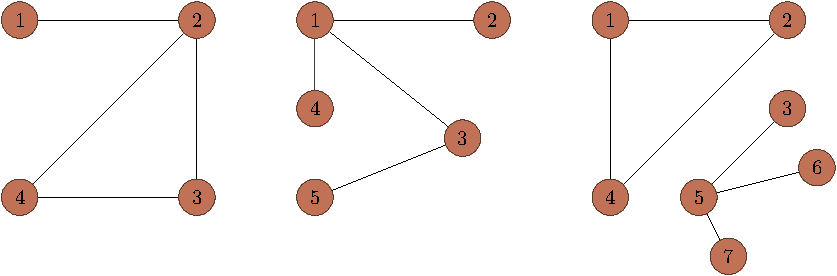
\includegraphics[width=\linewidth]{03_example_graph}
	
	\caption{\textbf{Przykłady grafów.} Cykliczny spójny (po lewej), acykliczny spójny (na środku), cykliczny niespójny (po prawej)\label{fig:example_graph}}
\end{figure}

Przykładowe grafy przedstawione sa na rysunku \ref{fig:example_graph}. Nas interesować będą jednak szczególne rodzaje grafów, nazywane drzewami.
\begin{df}[Charakteryzacja drzewa]
	Poniższe stwierdzenia są równoważne dla grafu $T = (N, E)$:
	\begin{enumerate}
		\item $T$ jest drzewem
		\item Dowolne dwa węzły grafu $T$ są połączone unikalną ścieżką w $T$.
		\item $T$ jest grafem spójnym, ale $T-e$ jest niespójnym dla dowolnej krawędzi $e\in E$
		\item $T$ jest grafem acyklicznym, ale $T +\{x,y\}$ będzie zawierać cykl dla dowolnych dwóch niesąsiadujących wierzchołków $x, y \in N$.
	\end{enumerate}
\end{df}

Jedynym drzewem widocznym na rysunku \ref{fig:example_graph} jest graf na środkowym panelu. Drzewa są istotne w teorii wielowymiarowych kopuł, ponieważ stanowią podstawowy element budujący \emph{regular vines}, czyli zbiory grafów które posłużą nam do przedstawiania struktury PCC.

\begin{df}[Regular vine]
	Zbiór drzew $\Nu = (T_1,\dots, T_{d-1})$ nazywamy \emph{regular vine}, lub \emph{R-vine} jeżeli:
	
	\begin{enumerate}
		\item Każde drzewo $T_j=(N_j, E_j)$ jest spójne
		\item $T_1$ jest drzewem o zbiorze wierzchołków $N_1$ i zbiorze krawędzi $E_1$
		\item Dla $j\geqslant2$, $T_j$ jest drzewem o zbiorze wierzchołków $N_j = E_{j-1}$ i zbiorze krawędzi $E_{j-1}$
		\item Dla $j = 2, \dots, d- 1$ oraz $\{a, b\} \in E_j$ mamy $ \vert a \cap b \vert = 1$. 
	\end{enumerate}
\end{df}

Na wykresie \ref{fig:r_vine} pokazujemy przykładową strukture R-vine. Opisu krawędzi i wierzchołków dokonujemy zgodnie z wprowadzanym poniżej pojęciem warunkowego i warunkowanego zbioru.

\begin{df}[Zbiór warunkowy, zbiór warunkowany]
	Dla dowolnej krawędzi $e\in E_i$ zdefiniujmy zbiór:
	$$ A_e\coloneqq \{j\in N_1\vert \exists e_1 \in E_1, \dots, e_{i-1}\in E_{i-1}: j\in e_1\in \dots \in e_{i-1}\in e\}.$$
	Zbiorem warunkującym $D_e$ krawędzi $e=\{a, b\}$ nazywamy:
	
	$$ D_e \coloneqq A_a \cup A_b,$$
	
	zbiorami warunkowanymi $C_{e, a}$ i $C_{e, b}$ nazywamy natomiast:
	
	$$ C_{e, a} \coloneqq A_a\\ D_e$$
	$$ C_{e, b} \coloneqq A_b\\ D_e.$$
	
	Skrótowo, będziemy opisywać krawędź $e = (C_{e, a}, C_{e, b}; D_e)$ jako $e = (e_a, e_b; D_e)$.
\end{df}


\begin{figure}[h]
	\centering
	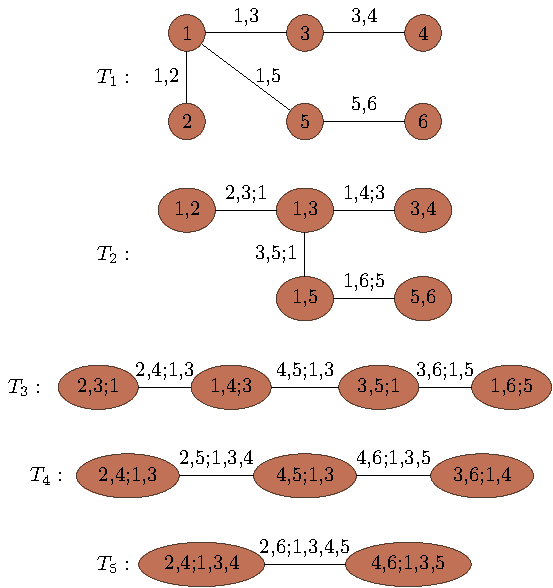
\includegraphics[width=0.7\linewidth]{03_R_vine}
	
	\caption{\textbf{Regular vine}. Przykładowa 6-wymiarowa struktura R-vine. \label{fig:r_vine}}
\end{figure}

Definicja struktury R-vine nie narzuca szczególnej postaci drzew. Jeżeli zaczniemy stawiać pewne warunki na ich strukturę, to trafimy w szczególności w dwie podklasy: D-vine i C-vine (rysunek \ref{fig:d_vine_c_vine}). D-vine zachodzi gdy każdy wierzchołek ma stopień co najwyżej równy dwa - powoduje to że drzewa wyglądają jak łańcuchy i nie mają odgałęzień. C-vine natomiast pojawia się w przypadku gdy każde drzewo ma pewien \emph{root node}, który jest połączony z każdym innym wierzchołkiem.
\begin{df}[D-vine, C-vine]
	Niech $\Nu$ będzie strukturą R-vine.
	\begin{enumerate}
		\item Jeżeli dla każdego wierzchołka $n\in N_i$ zachodzi warunek $\vert \{e\in E_i\vert n\in e\}\vert \leqslant 2$, to należy ona do podklasy \emph{D-vine} (drawable vine).
		\item Jeżeli dla każdego drzewa $T_i$ istnieje wierzchołek $n\in N_i$ taki, że $\vert \{e\in E_i\vert n\in e\}\vert = d-i$, to należy ona do podklasy \emph{C-vine} (canonical vine).
	\end{enumerate}
\end{df}


\begin{figure}[h]
	\centering
	\begin{minipage}{0.35\linewidth}
	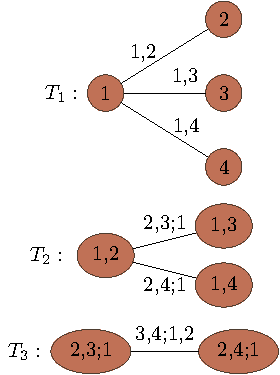
\includegraphics[width=\linewidth]{03_C_vine}
	\end{minipage}	
	\begin{minipage}{0.45\linewidth}
	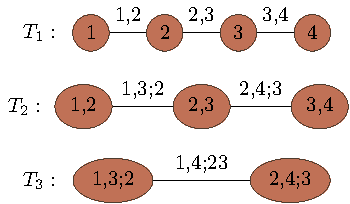
\includegraphics[width=\linewidth]{03_D_vine}
	\end{minipage}	

	\caption{\textbf{Canonical vine i Drawable vine.} Przykładowa 4-wymiarowa struktura C-vine (lewy panel) i D-vine (prawy panel).\label{fig:d_vine_c_vine}}
\end{figure}

Struktury R-vine są przydatne do wyjaśniania struktury zależności wielowymiarowych rozkładów, ponieważ jak pokazali \cite{BedfordCooke2002}, istnieje połączenie między PCC a pewnym R-vine.

\begin{df}[Rozkłady R-vine]
	Mówimy, że rozkład $F$ dla $d$-wymiarowego wektora losowego $(X_1, \dots, X_d)$ jest \emph{rozkładem R-vine}, jeśli możemy podać trójkę $(\mathcal{F}, \Nu, \mathcal{B})$ o własnościach:
	\begin{itemize}
		\item $\mathcal{F} =(F_1, \dots, F_d)$ jest wektorem ciągłych, odwracalnych dystrybuant rozkładów brzegowych $(X_1, \dots, X_d)$
		\item $\Nu$ jest $d$-wymiarową strukturą R-vine 
		\item Zbiór $\mathcal{B} = \{C_e\vert e \in E_i; i=1,\dots,d-1\}$, gdzie $C_e$ jest radialnie symetryczną dwuwymiarową kopułą posiadającą gęstość.
		\item Dla każdego $e\in E_i, i=1, \dots, d-1, e=\{a,b\}$, $C_e$ jest kopułą związaną z rozkładem warunkowym $X_{C_{e, a}}, X_{C_{e, b}}$ pod warunkiem $X_{D_e} = x_{D_e}$.
	\end{itemize}
	\label{def:r_vine_distribution}
\end{df}

W swojej pracy, Bedford i Cooke pokazują w szczególności, że dowolną trójkę $(\mathcal{F}, \Nu, \mathcal{B})$ o własnościach z definicji \ref{def:r_vine_distribution} można związać z pewnym $d$-wymiarowym rozkładem $F$.

\begin{thm}[Istnienie rozkładu R-vine]
	Niech $(\mathcal{F}, \Nu, \mathcal{B})$ spełnia warunki z definicji \ref{def:r_vine_distribution}. Wtedy istnieje dokładnie jeden $d$-wymiarowy rozkład $F$ o gęstości:
	
	\begin{equation*}
		\begin{split}
			f_{1, \dots, d}(x_1, \dots, x_d) = &f_1(x_1)\dots f_d(x_d) \cdot\\
			& \cdot \prod_{i=1}^{d-1}\prod_{e\in E_i}c_{C_{e, a}C_{e, b};D_e}(F_{C_{e, a}\vert D_e}(x_{C_{e, a}|x_{D_e}}), F_{C_{e, b}\vert D_e}(x_{C_{e, b}|x_{D_e}})),
		\end{split}
	\end{equation*}

	taki, że dla każdego $e\in E_i, i = 1,\dots, d-1$ oraz $e=\{a, b\}$ rozkład $X_{C_{e, a}}$ i $X_{C_{e,b}}$ pod warunkiem $X_{D_e} = x_{D_e}$ wyraża się poprzez:
	
	$$ F_{C_{e, a}C_{e, b}\vert D_e}(x_{C_{e, a}}, x_{C_{e, b}}|x_{D_e}) = C_{e}(F_{C_{e, a}\vert D_e}(x_{C_{e, a}|x_{D_e}}), F_{C_{e, b}\vert D_e}(x_{C_{e, b}|x_{D_e}})).$$
	
	Ponadto rozkłady brzegowe $F$ zadane są jako $F_i(x_i), i = 1,\dots, d.$
	\label{thm:existence_of_r_vine}
\end{thm}

Warunki z twierdzenia \ref{def:r_vine_distribution}, nie są znacząco restrykcyjne - jedynym potencjalnie problematycznym założeniem jest tu ciągłość rozkładów brzegowych i odwracalność dystrybuant. W praktyce więc można korzystać z wyniku \ref{thm:existence_of_r_vine} aby związać wielowymiarowy rozkład z reprezentacją R-vine.\\
Z twierdzenia \ref{thm:existence_of_r_vine} wynika nie tylko istnienie rozkładu R-vine, ale i również to, że dekompozycja używa kopuł związanych ze zbiorami warunkowymi obecnymi na grafie struktury R-vine i \emph{vice versa}. Z każdym wierzchołkiem i krawędzią struktury można więc związać pewien element dekompozycji - dwuwymiarową kopułę lub rozkład brzegowy. Wracając do przykładu z rozdziału \ref{subsub:przyklad_3_wymiary}, gdzie dla 3-wymiarowego rozkładu dostepne były trzy dekompozycje, możemy teraz zwizualizować te możliwości poprzez użycie struktury D-vine. Na rysunku \ref{fig:PCCs} widać, że dekompozycja zalezy jedynie od kolejności wymiarów w drzewie $T_1$.

\begin{figure}[h]
	\centering
	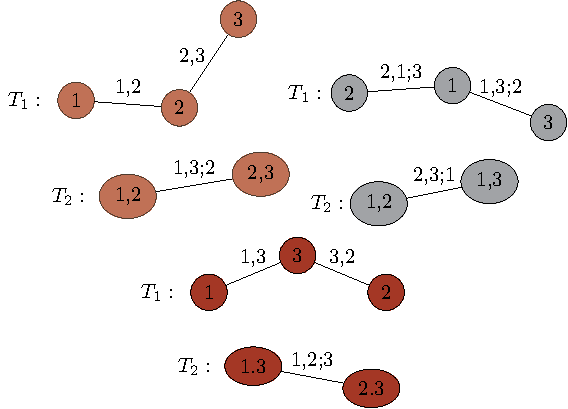
\includegraphics[width=0.8\linewidth]{03_PCC}
	
	\caption{\textbf{Pair Copula Constructions.} Trzy możliwe dekompozycje PCC 3-wymiarowego rozkładu, przedstawione w postaci R-vine. \label{fig:PCCs}}
\end{figure}

Widzimy zatem, że Vine Copula są przydatnym narzędziem pozwalającym na tworzenie bardzo elastycznych modeli, mających na celu lepsze, bardziej skrojone na wymiar uchwycenie struktury zależności w danych.\\
W kolejnym rozdziale opiszemy finansowe \emph{spready} będące funkcją ceny kilku aktywów rynkowych. Zaprezentujemy kilka sposobów na ich modelowanie, i pokażemy bardzo generalną metodę wykorzystującą Vine Copulas.
